\let\negmedspace\undefined
\let\negthickspace\undefined
\documentclass[journal]{IEEEtran}
\usepackage[a5paper, margin=10mm, onecolumn]{geometry}
%\usepackage{lmodern} % Ensure lmodern is loaded for pdflatex
\usepackage{tfrupee} % Include tfrupee package

\setlength{\headheight}{1cm} % Set the height of the header box
\setlength{\headsep}{0mm}     % Set the distance between the header box and the top of the text

\usepackage{gvv-book}
\usepackage{gvv}
\usepackage{cite}
\usepackage{amsmath,amssymb,amsfonts,amsthm}
\usepackage{algorithmic}
\usepackage{graphicx}
\usepackage{textcomp}
\usepackage{xcolor}
\usepackage{txfonts}
\usepackage{listings}
\usepackage{enumitem}
\usepackage{mathtools}
\usepackage{gensymb}
\usepackage{comment}
\usepackage[breaklinks=true]{hyperref}
\usepackage{tkz-euclide} 
\usepackage{listings}
% \usepackage{gvv}                                        
\def\inputGnumericTable{}                                 
\usepackage[latin1]{inputenc}                                
\usepackage{color}                                            
\usepackage{array}                                            
\usepackage{longtable}                                       
\usepackage{calc}                                             
\usepackage{multirow}                                         
\usepackage{hhline}                                           
\usepackage{ifthen}                                           
\usepackage{lscape}
\usepackage{circuitikz}
\tikzstyle{block} = [rectangle, draw, fill=blue!20, 
    text width=4em, text centered, rounded corners, minimum height=3em]
\tikzstyle{sum} = [draw, fill=blue!10, circle, minimum size=1cm, node distance=1.5cm]
\tikzstyle{input} = [coordinate]
\tikzstyle{output} = [coordinate]




\bibliographystyle{IEEEtran}
\vspace{3cm}

\title{5.2.2}
\author{AI25BTECH11039-Harichandana Varanasi}
 \maketitle
% \newpage
% \bigskip
{\let\newpage\relax\maketitle}

\renewcommand{\thefigure}{\theenumi}
\renewcommand{\thetable}{\theenumi}
\setlength{\intextsep}{10pt} % Space between text and floats


\numberwithin{equation}{enumi}
\numberwithin{figure}{enumi}
\renewcommand{\thetable}{\theenumi}



\date{}

\begin{document}
\maketitle


\noindent\textbf{Question.}\;
Solve the simultaneous linear equations
\[
5u-4v+8=0,\qquad 7u+6v-9=0 .
\]
\renewcommand\theequation{\arabic{equation}}
\begin{align}
5u - 4v &= -8 \tag{1}\\
7u + 6v &= 9 \tag{2}
\end{align}

Writing in matrix form,
\begin{equation}
\myvec{5 & -4 \\ 7 & 6}\myvec{u \\ v}=\myvec{-8 \\ 9} \tag{3}
\end{equation}

Augmented matrix,
\begin{equation}
\myvec{5 & -4 & -8 \\ 7 & 6 & 9} \tag{4}
\end{equation}

\noindent Row operation: $R_2 \to 5R_2 - 7R_1$,
\begin{equation}
\myvec{5 & -4 & -8 \\ 0 & 58 & 101} \tag{5}
\end{equation}

\noindent Normalize second row: $R_2 \to \dfrac{R_2}{58}$,
\begin{equation}
\myvec{5 & -4 & -8 \\ 0 & 1 & \dfrac{101}{58}} \tag{6}
\end{equation}

\noindent Eliminate above: $R_1 \to R_1 + 4R_2$,
\begin{equation}
\myvec{5 & 0 & -\dfrac{30}{29} \\ 0 & 1 & \dfrac{101}{58}} \tag{7}
\end{equation}

\noindent Normalize first row: $R_1 \to \dfrac{R_1}{5}$,
\begin{equation}
\myvec{1 & 0 & -\dfrac{6}{29} \\ 0 & 1 & \dfrac{101}{58}} \tag{8}
\end{equation}

Thus, the solution vector is
\begin{equation}
\myvec{u \\ v}=\myvec{-\dfrac{6}{29} \\ \dfrac{101}{58}} \tag{9}
\end{equation}



\clearpage                       
\begin{figure}[H]
  \centering
  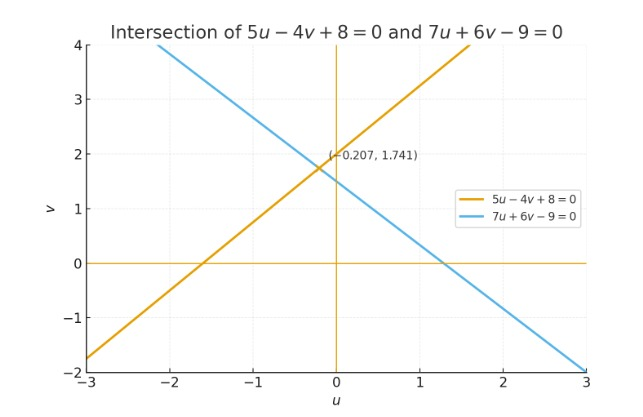
\includegraphics[width=0.8\linewidth]{figs/matgeo-5.2.2.jpeg}
  \caption{Intersection of $5u-4v+8=0$ and $7u+6v-9=0$ at
           $\left(-\tfrac{6}{29},\,\tfrac{101}{58}\right)$.}
  \label{fig:5.2.2}
\end{figure}





 

\end{document}
